\section{动量 II \& 动能与势能}

\subsection{质点系的动量变化}

\begin{theorem}[质点系的动量变化定理]
    对于一个质点系，设 $\vect{F}_i$ 为质点 $i$ 受到的合外力，$\vect{f}_{i, j}$ 为质点 $i$ 收到质点 $j$ 的作用力，那么
    $$
    \dd \vect{P} = \sum_{i=1}^n \dd \vect{p}_i = \sum_{i=1}^n \vect{F}_i \dd t
    $$
\end{theorem}

\begin{theorem}[动量守恒定律]
    惯性系中，如果一个质点系的合外力为零，那么它的总动量守恒。
\end{theorem}

动量守恒也可以仅在其中一个方向上成立。如沿 $x$ 轴的合外力为零，那么 $\vect{P}_x$ 守恒。

\subsection{功、功率}

质点 $m$ 在从 $\vect{a} \to \vect{b}$ 的运动过程有变力 $F$，那么该过程中力做的功为
$$
W = \int_{\vect{a}}^{\vect{b}} \vect{F} \cdot \dd{\vect{r}}
$$
其中 $\vect{r}$ 是质点的位移。这是一个线积分，得到一个标量。

合力做的功等于各分力的功之和。

\subsection{作业}

\begin{problem}
    习题 2.1
    \begin{solution}
        不妨设杆 $AB$ 质量为 $m$，那么杆的加速度为 $\vect{a} = \frac{1}{m} \ab(\vect{f}_1 + \vect{f}_2)$。设 $AC$ 对 $CB$ 的作用力为 $\vect{F}$。
        \begin{itemize}
            \item 对 $AC$ 分析：$\vect{f}_1 - \vect{F} = \frac{1}{n} m \vect{a}$。
            \item 对 $CB$ 分析：$\vect{f}_2 + \vect{F} = \frac{n-1}{n} m \vect{a}$。
        \end{itemize}
        解得 $\vect{F} = \frac{n - 1}{n} \vect{f}_1 - \frac{1}{n} \vect{f}_2$。
    \end{solution}
\end{problem}

\begin{problem}
    习题 2.3
    \begin{solution}
        取 $\ab{\vect{g}} = 10\,\mathrm{m / s^2}$。
        \begin{enumerate}
            \item[\textbf{1)}] 设板对物体的摩擦力大小为 $f_2$，桌面对板的摩擦力大小为 $f_3$，那么
            $$
            \begin{dcases}
                F_1 - f_3 = (m + M) a \\
                f_2 = m a \\
                f_3 = \mu (M + m) g
            \end{dcases}
            $$
            解得 $f_2 = 2 \,\mathrm{N}, f_3 = 7.5\,\mathrm{N}$。这是水平方向的作用力。

            垂直方向有支持力，板与物体之间的支持力为 $20 \,\mathrm{N}$，板与桌面之间的支持力为 $30 \,\mathrm{N}$。

            \item[\textbf{2)}] 设恰好抽出时的力为 $F$，那么：
            $$
            \begin{dcases}
                f_2' = \mu m g \\
                f_3' = \mu (m + M) g \\
                \frac{F - f_3'}{m + M} = \frac{f_2'}{m}
            \end{dcases}
            $$
            解得 $F = 15 \,\mathrm{N}$。
        \end{enumerate}
    \end{solution}
\end{problem}

\begin{problem}
    习题 2.9
    \begin{solution}
        由题可知
        $$
        m \dd{\vect{v}} = \vect{F} \dd{t} = -k \vect{v} \dd{t}
        $$
        推导得到：
        $$
        \begin{gathered}
            \int_0^t \frac{m \dd{\vect{v}}}{\vect{v}} = \int_0^t -k \dd{t} \\
            \implies m \ln \frac{\vect{v}}{\vect{v}_0} = -k t \\
            \implies \vect{v} = \vect{v}_0 \mathrm{e}^{-\frac{k}{m} t}
        \end{gathered}
        $$
    \end{solution}
\end{problem}

\begin{problem}
    习题 2.14
    \begin{solution}
        对于绳上一个距离轴 $r$ 的微元 $\dd{m} = m \cdot \frac{\dd{r}}{l}$，有
        $$
        \begin{aligned}
            & & T(r) - T(r + \dd{r}) & = \dd{m} r \omega^2 \\
            \implies & & \dd{T} & = \frac{m \omega^2 r}{l} \dd{r} \\
            \implies & & \int_{T(l)}^{T(R)} \dd{T} & = \int_l^R \frac{m \omega^2 r}{l} \dd{r} \\
            \implies & & T(R) & = \frac{m \omega^2}{2l} (l^2 - R^2)
        \end{aligned}
        $$
    \end{solution}
\end{problem}

\begin{problem}
    习题 2.20
    \begin{solution}
        \begin{itemize}
            \item 机内：在机内参考系 $B$ 受惯性力 $\vect{F}_0 = -m \vect{a} = \frac{1}{2} m \vect{g}$，合力为 $\vect{F} = \vect{F}_0 + m \vect{g} = \frac{3}{2} m \vect{g}$。因此 $A, B$ 的加速度为 $\abs{\vect{a}_1} = \abs{\frac{\vect{F}}{2m}} = \frac{3}{4} \abs{\vect{g}}$。
            \item 机外：观察到 $A$ 的加速度为 $\abs{\vect{a}_A} = \abs{\vect{a}_1 + \vect{a}} = \frac{\sqrt{13}}{4} \abs{\vect{g}}$，$B$ 的加速度为 $\abs{\vect{a}_B} = \abs{\vect{a}_1 + \vect{a}} = \frac{1}{4} \abs{\vect{g}}$。
        \end{itemize}
    \end{solution}    
\end{problem}

\begin{problem}
    习题 2.22
    \begin{solution}
        \begin{itemize}
            \item 真实力：$F_1 = m R \omega^2$，方向指向圆心。
            \item 惯性力：惯性离心力 $F_2 = m R \omega^2$，方向背离圆心。
        \end{itemize}
    \end{solution}
\end{problem}

\begin{problem}
    习题 2.23
    \begin{solution}
        地球自转自西向东，列车受科里奥利力方向向东，故铁轨东侧受压力。

        \begin{figure}[H]
            \centering
            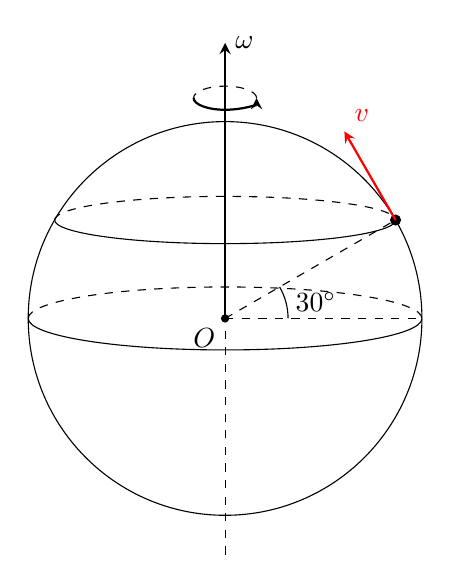
\begin{tikzpicture}[>=stealth]
                \def\R{2.5}
                \def\ang{30}
                
                % 地球轮廓
                \draw (0,0) circle (\R);
                \fill (0,0) circle (1.5pt) node[below left] {$O$};
                
                % 赤道
                \draw (\R,0) arc (0:-180:{\R} and 0.4);
                \draw[dashed] (-\R,0) arc (180:0:{\R} and 0.4);
                
                % 北半球30度纬线
                \draw ({\R*cos(\ang)},{\R*sin(\ang)}) arc (0:-180:{\R*cos(\ang)} and 0.3);
                \draw[dashed] ({-\R*cos(\ang)},{\R*sin(\ang)}) arc (180:0:{\R*cos(\ang)} and 0.3);
                
                % 自转轴
                \draw[dashed] (0,-3) -- (0,0);
                \draw[->, thick] (0,0) -- (0,3.5) node[right] {$\vect{\omega}$};
                
                % 自转方向
                \draw[->, thick] (-0.4, 2.8) arc (180:360:0.4 and 0.15);
                \draw[dashed] (0.4, 2.8) arc (0:180:0.4 and 0.15);
                
                % 角度标示
                \draw[dashed] (0,0) -- (\R,0);
                \coordinate (P) at ({\R*cos(\ang)}, {\R*sin(\ang)});
                \draw[dashed] (0,0) -- (P);
                \draw (0.8,0) arc (0:\ang:0.8) node[midway, right] {$30^\circ$};
                
                % 列车
                \fill (P) circle (2pt) node[right, xshift=2pt] {};
                
                % 速度方向 (沿着切线向北)
                \draw[->, thick, red] (P) -- ++(120:1.3) node[above right] {$\vect{v}$};
            \end{tikzpicture}
            \caption{题目图示}
        \end{figure}

        侧压力大小为：
        $$
        \begin{aligned}
            \abs{\vect{F}} & = \abs{2m \vect{v} \times \vect{\omega}} \\
            & = 2m \cdot \abs{\vect{v}} \cdot \abs{\omega} \sin 30^\circ \\
            & = 2 \times 5 \times 10^4 \,\mathrm{kg} \times \frac{9 \times 10^4 \,\mathrm{m}}{3.6 \times 10^3 \,\mathrm{s}} \times \frac{2\pi}{24 \times 3600 \,\mathrm{s}} \times \frac{1}{2} \\
            & = 90.90 \,\mathrm{N}
        \end{aligned}
        $$
    \end{solution}
\end{problem}

\begin{problem}
    习题 3.3
    \begin{solution}
        $$
        \begin{dcases}
            I = m \sqrt{2gh} \\
            \frac{I}{\Delta t} \ge \mu_0 M g
        \end{dcases}
        $$
        解得 $h \ge \frac{\mu_0^2 M^2 g^2 (\Delta t)^2}{2 m^2}$。
    \end{solution}
\end{problem}

\begin{problem}
    习题 3.5
    \begin{solution}
        恰好打断时有：
        $$
        \begin{dcases}
            I = m v \\
            \frac{m v^2}{l} = T_0 - m g
        \end{dcases}
        $$
        解得 $I = 0.86 \,\mathrm{N \cdot s}$。
    \end{solution}
\end{problem}
